
\فصل{مفاهیم اولیه}
در این فصل مفاهیم اولیه لازم برای فهم مسأله و نتایج پایان نامه را مطرح میکنیم. ابتدا نحوه پردازش تراکنش ها در بلاکچین بیتکوین را توضیح میدهیم و سپس توضیح میدهیم که تراکنش های یک کانال پرداخت چه تفاوتی با تراکنش های عادی درون بلاکچینی دارند و چگونه میتوان تراکنش برون بلاکچینی امن داشت. در این بخش هنگام توضیح جزئیات پروتکل ها بلاکچین بیتکوین و شبکه کانال های پرداخت آن یعنی \کد{Lightning network} را به عنوان معیار در نظر میگیریم زیرا اولا امروزه \کد{Lightning network} با داشتن بیش از 17000 نود، پرکاربر ترین شبکه کانال های پرداخت موجود است 
~\cite{1ml}
و ثانیا مفاهیم پایه ای تراکنش های درون بلاکچینی و برون بلاکچینی کمابیش برای تمام بلاکچین ها یکسان است و تنها تفاوت در پروتکل های پیاده سازی شده است، پس تفاوت چندانی ندارد که کدام بلاکچین را به عنوان معیار قرار دهیم. 

\قسمت{تراکنش ها در بیتکوین}
بیتکوین یک بلاکچین \کد{UTXO-based} است، در این سیستم هر تراکنش یک یا تعدادی ورودی و یک یا تعدادی خروجی دارد. در هر تراکنش مجموع بیتکوین ورودی ها برابر است با مجموع بیتکوین خروجی ها و کارمزد تراکنش. شکل \رجوع{شکل:تراکنش} را ببینید. هر تراکنش یک هش \پاورقی{hash} یکتا دارد که شناسه تراکنش محسوب میشود. 
هر کدام از ورودی های یک تراکنش یکی از خروجی های یک تراکنش قدیمی تر را خرج میکند. هر خروجی دو داده در بر دارد : 1)مقدار پول موجود در آن 2) یک کد قفل کننده (\کد{ScriptPubKey}) که کلید عمومی \پاورقی{public key} و سایر مشخصات کسی که میتواند خروجی را خرج کند مشخص میکند. 
مثلا در شکل \رجوع{شکل:تراکنش} به خروجی شماره $1$ تراکنش سمت چپ دقت کنید. این خروجی دو بیتکوین دارد و  کد قفل کننده \کد{ScriptPubKey\_1}، کلید عمومی کسی که میتواند این پول را خرج کند مشخص میکند. این خروجی توسط ورودی شماره $1$ تراکنش سمت راست خرج میشود. 
هر ورودی سه داده را در بر دارد 1) هش تراکنشی که میخواهد یکی از خروجی های آن را خرج کند (در این مثال هش تراکنش سمت چپ که با قرمز رنگ مشخص شده است) 2) شماره خروجی مورد نظر( در این مثال، عدد $1$ که با سبز رنگ مشخص شده است ) 3) یک کد باز کننده قفل که شامل امضای صاحب پول و سایر اثبات های مورد نیاز  خروجی است (در این مثال، \کد{ScriptSig\_1} که با رنگ سرمه ای مشخص شده است) .  همچنین دقت کنید که در تراکنش سمت راست ورودی $2$ بیتکوین دارد و مجموع خروجی ها $1.99$ بیتکوین است؛ $0.01$ بیتکوین هم به عنوان کارمزد شبکه در نظر گرفته شده است.

 

\شروع{شکل}[hb]
\centerimg{tx}{11cm}
\شرح{ساختار یک تراکنش در بیتکوین}
\برچسب{شکل:تراکنش}
\پایان{شکل}


توجه کنید که کد قفل کننده و باز کننده قفل باید سازگار باشند مثلا دو عبارت زیر سازگار هستند:

\شروع{شکل}[hb]
\centerimg{lock1.png}{6cm}
\پایان{شکل}

کد قفل کننده میتواند شروط بیشتر و پیچیده تری هم برای خرج کننده خروجی ایجاب کند. مثلا به کد قفل کننده و بازکننده زیر توجه کنید که به امضای هر دو کاربر \کد{A}  و  \کد{B} نیازدارد. این خروجی مانند یک حساب دو کاربره عمل میکند زیرا برای خرج کردن پول آن تایید هر دو کاربر \کد{A}  و  \کد{B} لازم است.
%همچنین برای استفاده از این خروجی باید حداقل 5 دقیقه از تایید شدن این تراکنش گذشته باشد.

\شروع{شکل}[h]
\centerimg{lock2.png}{9cm}
\پایان{شکل}

\paragraph{قفل زمانی}
تراکنش های بیتکوین میتوانند شامل جزئیات دیگری مانند قفل زمانی\پاورقی{time lock} هم باشند. قفل زمانی به این معنی است که یک تراکنش را پیش از زمان مقرر نمیتوان به بلاکچین ارسال کرد. به طور مثال اگر شما تراکنشی با قفل زمانی \کد{December 31} بسازید و آن را پیش از این تاریخ به بلاکچین ارسال کنید، ماینر ها این تراکنش را ثبت نمیکنند و تا روز \کد{December 31} صبر کرده و بعد آن را ثبت میکنند.

\paragraph{خروجی های خرج نشده}
\پاورقی{UTXO}
به خروجی هایی که تاکنون خرج نشده اند \کد{Unspent Transaction Output (UTXO)} میگویند.  ماینر\پاورقی{miner} ها در شبکه بیتکوین دو وظیفه اصلی دارند:
\شروع{شمارش}
\فقره
 اطمینان حاصل کنند که هیچ خروجی ای بیش از یکبار خرج نمیشود .
\فقره
 بررسی کنند که هر کد باز کننده به درستی کد قفل کننده متناظر را باز میکند.
\پایان{شمارش}

\قسمت{تراکنش های کانال پرداخت}\برچسب{قسمت:تراکنش های کانال پرداخت}

در این بخش نوع ساخت و استفاده از کانال پرداخت های بر مبنای زمان\پاورقی{time based payment channels} ها را توضیح میدهیم. کانال پرداخت های رایج در \کد{Lightning Network} معمولا از نوع \کد{punishment based payment channel} هستند که  جزئیات پیچیده تری نسبت به کانال های بر مبنای زمان دارند. با این وجود چون اصول اولیه و کلیات هر دو این پروتکل ها مشابه هم است، فهم اصول کانال های بر مبنای زمان کافی است. برای خواندن درباره تفاوت این دو پروتکل ایجاد کانال میتوانید به منبع
~\cite{paymentChannBlog} 
مراجعه کنید.


\subsection{ایجاد کانال}
همانطور که پیش از این گفته شد، دو کاربر برای ایجاد کانال پرداخت باید یک تراکنش درون بلاکچینی "ایجاد کانال" بسازند. شکل \رجوع{شکل:تراکنش ایجاد کانال} تراکنش \کد{Tx1} را نشان میدهد که نمونه ای از یک تراکنش ایجاد کانال است. \کد{A} یکی از \کد{UTXO} هایش به ارزش $2$ بیتکوین و B یکی از \کد{UTXO} هایش به ارزش $4$ بیتکوین را در کانال سپرده میکنند. خروجی \کد{Tx1} یک \کد{UTXO} دو کاربره با موجودی 6 است. 

\شروع{شکل}[h]
\centerimg{channelCreation.png}{8cm}
\شرح{مثالی از یک تراکنش ایجاد کانال پرداخت. این تراکنش درون بلاکچینی است یعنی روی بلاکچین بیتکوین فرستاده میشود.}
\برچسب{شکل:تراکنش ایجاد کانال}
\پایان{شکل}
\subsection{استفاده از کانال}
همزمان یا اندکی پیش از امضای تراکنش درون بلاکچینی \کد{Tx1}، \کد{A}  و  \کد{B} مشترکا یک تراکنش برون بلاکچینی (\کد{Tx2}) هم ساخته و هر دو آن امضا میکنند اما آن را روی بلاکچین نمیفرستند، این تراکنش تنها در حافظه محلی \کد{A}  و  \کد{B} ذخیره میشود. 

\شروع{شکل}[h]
\centerimg{state0.png}{6cm}
\شرح{تراکنش حالت صفر کانال پرداخت. این تراکنش برون بلاکچینی است یعنی توسط \کد{A}  و  \کد{B} مشترکا ساخته و امضا شده و ذخیره می شود ولی تا زمان بسته شدن کانال روی بلاکچین قرار نمیگیرد.}
\برچسب{شکل:تراکنش حالت صفر}
\پایان{شکل}



\کد{Tx2} تک خروجی تراکنش \کد{Tx1} را خرج میکند و ، پول موجود در کانال را به همان نسبت اولیه $2-4$ بین \کد{A}  و  \کد{B} تقسیم میکند.
% برای استفاده از  خروجی \کد{Tx2} حداقل 30 روز از ثبت آن در بلاکچین باید گذشته باشد. 
تراکنش \کد{Tx2} تنها پس از زمان مقرر قفل زمانی(در این مثال \کد{December 31}) بر بلاکچین ثبت میشود.
\کد{Tx2} در واقع توزیع پول در کانال را در لحظه ایجاد آن یا لحظه صفر نشان میدهد به همین دلیل به آن تراکنش لحظه صفر میگوییم. در صورتی که هیچ تراکنشی بین \کد{A}  و  \کد{B}  انجام نگیرد و پس از مدتی یکی از \کد{A}  یا  \کد{B} تصمیم بگیرد کانال را ببندد، آن فرد میتواند تراکنش \کد{Tx2} را روی بلاکچین قرار دهد. چون \کد{Tx2}  پیش از این توسط هر دو \کد{A}  و  \کد{B} امضا شده است پس تراکنش معتبری است و بعد از تاریخ  قفل زمانی آن \کد{A}  و  \کد{B}  هر کدام میتوانند سهم خود را از کانال پرداخت بگیرند و کانال بسته میشود. اما در عمل \کد{A}  و  \کد{B}  کانال پرداخت ساخته اند تا از آن استفاده کنند نه اینکه آن را بلافاصله ببندند پس تراکنش \کد{Tx2} عملا هیچگاه استفاده نمیشود. این تراکنش تنها و تنها ساخته میشود تا به هر دو طرف تضمین دهد که اگر طرف دیگر پاسخگو نبود، پول آن ها در کانال قفل نمیماند و هر کدام میتوانند سهم خود را از کانال دریافت کنند.

اکنون با یک مثال توضیح میدهیم که در عمل چگونه از کانال پرداخت ایجاد شده در شکل \رجوع{شکل:تراکنش ایجاد کانال} استفاده میشود. فرض کنید  \کد{B} میخواهد برای \کد{A} 1 بیتکوین در کانال پول بریزد. \کد{B} تراکنش برون بلاکچینی \کد{Tx3} نمایش داده شده در شکل \رجوع{شکل:تراکنش حالت یک} را میسازد و امضا میکند و برای \کد{A} میفرستد. \کد{A} هم \کد{Tx3} را امضا کرده و ذخیره میکند. \کد{Tx3} توزیع پول موجود در کانال را به $3-3$ تغییر میدهد. هرگاه هر کدام از  \کد{A}  یا  \کد{B} بخواهند این کانال را ببندند کافی است \کد{Tx3} را روی بلاکچین بفرستد و در تاریخ \کد{December 30} سهم خود از کانال را پس بگیرند. 

\شروع{شکل}[h]
\centerimg{state1.png}{6cm}
\شرح{}
\برچسب{شکل:تراکنش حالت یک}
\پایان{شکل}

اما یک مشکل وجود دارد؛ چگونه تضمین دهیم که هیچ کدام از طرفین تراکنش قدیمی تر \کد{Tx2} را روی بلاکچین قرار نمیدهند تا کانال را با یک توزیع پول قدیمی ببندند؟ دقت کنید که هر دو \کد{Tx2} و \کد{Tx3} تک خروجی تراکنش \کد{Tx1} را خرج میکنند بنابراین فقط یکی از آن ها قابل اجرا روی بلاکچین است. محدودیت زمانی اعمال شده روی خروجی تراکنش های \کد{Tx2} و \کد{Tx3} تضمین کننده این است که تراکنشی که دیرتر تولید شده است، \کد{Tx3}، زودتر اجرا خواهد شد؛ با یک مثال این موضوع را توضیح میدهیم. فرض کنید \کد{A} میخواهد سر \کد{B} کلاه بگذارد و بدون هیچ اطلاع قبلی تراکنش \کد{Tx2} را روی بلاکچین قرار میدهد؛ \کد{B} با دیدن این عمل، تراکنش  \کد{Tx3}  را به بلاکچین میفرستد. قفل زمانی  \کد{Tx3} روز \کد{December 30} باز میشود پس این تراکنش یک روز زودتر از \کد{Tx2} قابل اجرا است. تراکنش  \کد{Tx3} در روز \کد{December 30} انجام میشود و بعد از آن، تراکنش \کد{Tx2} دیگر قابل اجرا نخواهد بود زیرا ورودی آن قبلا توسط  \کد{Tx3} مصرف شده است.

منطق مشابهی در تمام مدت استفاده از کانال استفاده میشود مثلا اگر روز بعد \کد{B} بخواهد به \کد{A} 2 بیتکوین بدهد، باید تراکنش \کد{Tx4} را تولید کند و امضا کرده و برای او بفرستد.

\شروع{شکل}[h]
\centerimg{state2.png}{6cm}
\شرح{}
\برچسب{شکل:تراکنش حالت دو}
\پایان{شکل}

در نهایت وقتی طرفین تصمیم بگیرند کانال پرداخت را ببندند، آخرین تراکنش را روی بلاکچین میفرستند یعنی در نهایت فقط یکی از تراکنش های \کد{Tx2} \کد{Tx3}  \کد{Tx4} اجرا میشود. همانطور که در بالا توضیح دادیم، قفل زمانی کاهنده تراکنش ها تضمین میکند که همیشه جدید ترین تراکنش اجرا شود.

\شروع{شکل}[h]
\centerimg{channelClosure.png}{13cm}
\شرح{بستن کانال پرداخت}
\برچسب{شکل:تراکنش بستن کانال}
\پایان{شکل}

شکل \رجوع{شکل:تراکنش بستن کانال} نشان میدهد که چطور تراکنش \کد{Tx4} با خرج کردن تک خروجی \کد{Tx1}، کانال پرداخت را میبندد. مجددا دقت کنید که تراکنش  \کد{Tx4} در ابتدا برون بلاکچینی بود ولی در نهایت چون آخرین تراکنش بود روی بلاکچین قرار گرفت و درون بلاکچینی شد اما سایر تراکنش ها یعنی \کد{Tx2} و \کد{Tx3} برون بلاکچینی هستند و پیش از بستن کانال میتوان تا زمانی که موجودی طرفین اجازه میدهد بیشماره تراکنش برون بلاکچینی داشت.



\قسمت{تراکنش های با واسطه} همانطور که در قسمت قبل توضیح دادیم، با ایجاد یک کانال پرداخت دو کاربر \کد{A} و \کد{B} میتوانند تنها با دو تراکنش درون بلاکچینی تعداد دلخواهی تراکنش برون بلاکچینی برای هم بفرستند اما همچنان محدودیت این روش این است که کاربران دو به دو باید کانال پرداخت ایجاد کنند. برای حل این مشکل توسعه دهندگان Lightning Network پروتکلی طراحی کرده اند که این امکان را به کاربران میدهد که با یک یا چندین واسطه تراکنش برای هم بفرستند
~\cite{poon2015lightning}.
تراکنش با واسطه را با یک مثال توضیح میدهیم. به شکل \ref{شکل: تراکنش با واسطه} توجه کنید، کاربر \کد{A} و \کد{B} با هم و کاربر \کد{B} و \کد{C} با هم کانال دارند و کاربر \کد{A} میخواهد با استفاده از  \کد{B} به عنوان واسطه برای \کد{C} 1 بیتکوین بفرستد. در شکل \ref{شکل:تراکنش با واسطه مرحله یک} 
که مرحله اول را نشان میدهد میتوانید موجودی هر فرد در کانال ها پیش از انجام تراکنش را ببینید. در این مرحله \کد{C} یک مقدار تصادفی و محرمانه
$r$
را انتخاب کرده و آن را از یک تابع چکیده ساز \پاورقی{Hash function}، که در اینجا با 
$H(.)$
نمایش داده شده است عبور میدهد تا 
$h$
حاصل شود و بعد
$h$ 
را برای \کد{A} ارسال میکند. در اینجا لازم است توضیح مختصری درباره توابع چکیده ساز بدهیم. این توابع یک ورودی از طول دلخواه را گرفته و به خروجی به طول معین تبدیل میکنند. در حالیکه محاسبه این توابع از نظر محاسباتی ساده است اما محاسبه وارون آن ها دشوار است بنابراین با داشتن 
$h$
محاسبه 
$r$
ممکن نیست.

در مرحله دو که در شکل \ref{شکل:تراکنش با واسطه مرحله دو} نمایش داده شده،  \کد{A}  یک تراکنش 1 بیتکوینی برای  \کد{B} میفرستد اما شرط اینکه این تراکنش اجرا شود این است که  \کد{B} بتواند پیش از زمان معین \کد{timeout}
$r$
را طوری پیدا کند که 
$H(r)=h$
سپس \کد{B} تراکنش مشابهی را منتها با  \کد{timeout} کوتاه تر تولید کرده و برای \کد{C} میفرستد. تنها کسی که
$r$
را میداند \کد{C} است پس پیش از به پایان رسیدن \کد{timeout} \کد{C}، 
$r$
را برای \کد{B} فرستاده (شکل \ref{شکل:تراکنش با واسطه مرحله سه}) و قفل تراکنش باز میشود و 1 بیتکوین به صورت برون بلاکچینی از \کد{B} به \کد{C} واریز میشود. سپس چون \کد{timeout} تراکنش  \کد{A-B} بیشتر از  \کد{timeout} تراکنش  \کد{B-C} است \کد{B} زمان کافی خواهد داشت که 
$r$
را برای \کد{A} بفرستد و 1 بیتکوین خود را از او بگیرد (شکل \ref{شکل:تراکنش با واسطه مرحله چهار}) و به این ترتیب \کد{B} همان پولی را که در کانال با \کد{C} از دست میدهد در کانال با \کد{A}  بدست می آورد.  اگر زمان \کد{timeout}  هر کدام از تراکنش ها بگذرد آن تراکنش کلا برگشت میخورد پس اگر  \کد{C} آفلاین شود و نتواند
$r$
را تا پیش از \کد{timeout} نفرستد، تراکنش \کد{B-C} برگشت میخورد و بالطبع چون  \کد{B} هم به هیچ وجه نمیتواند 
$r$
را پیدا کند، تراکنش  \کد{A-B} هم برگشت میخورد به همین دلیل میگوییم این تراکنش ها \کد{atomic} هستند یعنی یا هر دو با هم انجام میشوند یا هر دو برگشت میخورند.

  
\begin{figure}
     \centering
     \begin{subfigure}[b]{0.48\textwidth}
         \centering
	\centerimg{intermediary1.png}{7cm}
         %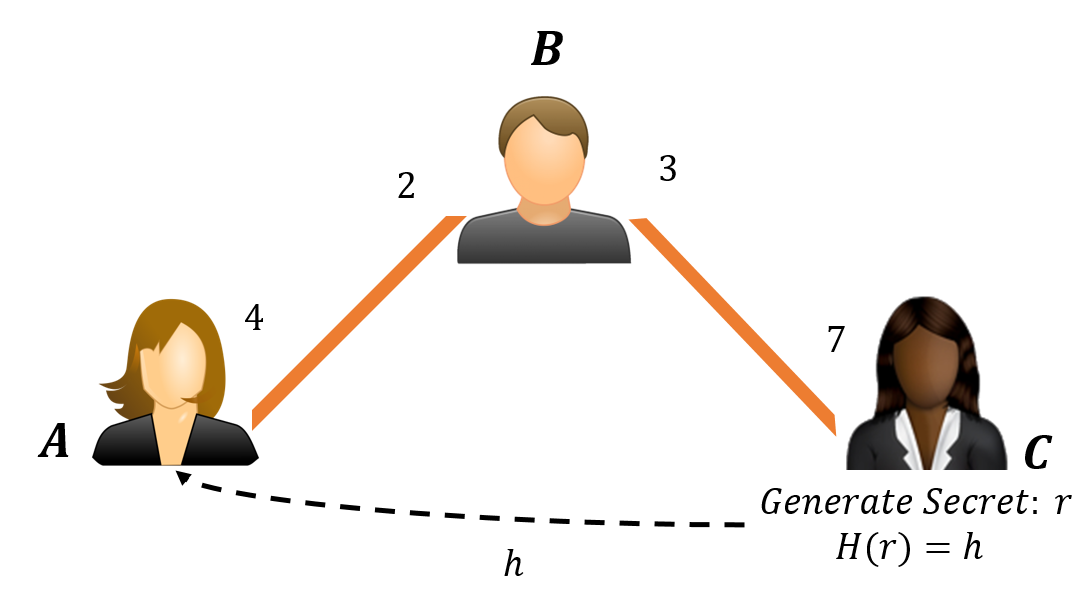
\includegraphics[width=3cm]{intermediary1.png}
         \caption{}
         \label{شکل:تراکنش با واسطه مرحله یک}
     \end{subfigure}
     \hfill
     \begin{subfigure}[b]{0.48\textwidth}
         \centering
	\centerimg{intermediary2p.png}{7cm}
         %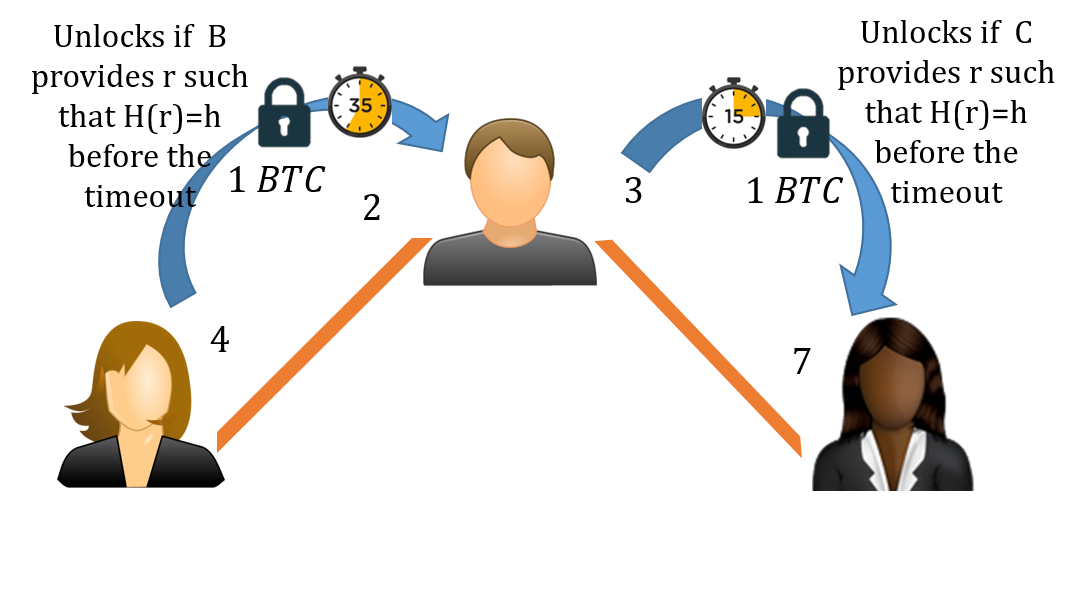
\includegraphics[width=\textwidth]{intermediary2p.png}
         \caption{}
         \label{شکل:تراکنش با واسطه مرحله دو}
     \end{subfigure}


\begin{subfigure}[b]{0.48\textwidth}
         \centering
	\centerimg{intermediary3p.png}{7cm}
         %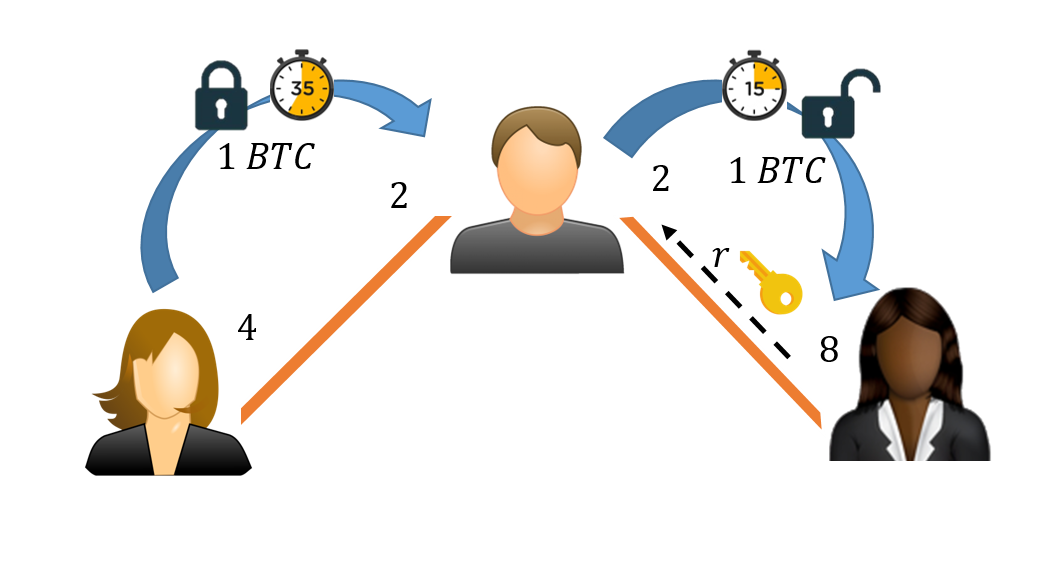
\includegraphics[width=\textwidth]{intermediary3p.png}
         \caption{}
         \label{شکل:تراکنش با واسطه مرحله سه}
     \end{subfigure}
     \hfill
     \begin{subfigure}[b]{0.48\textwidth}
         \centering
	\centerimg{intermediary4p.png}{7cm}
         %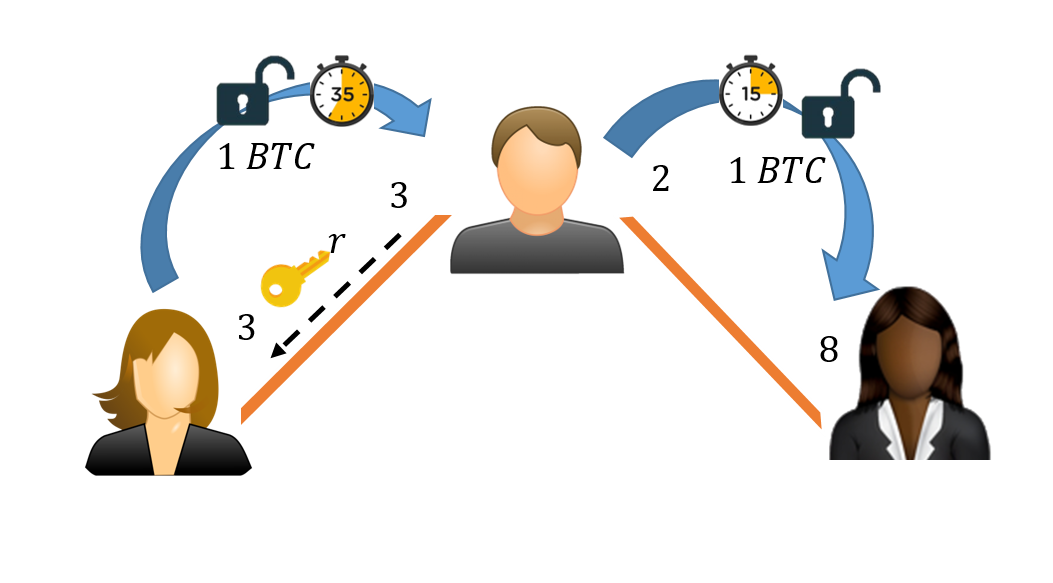
\includegraphics[width=\textwidth]{intermediary4p.png}
         \caption{}
         \label{شکل:تراکنش با واسطه مرحله چهار}
     \end{subfigure}
        \caption{مراحل انجام یک تراکنش با واسطه در شبکه کانال های پرداخت}
        \label{شکل: تراکنش با واسطه}
\end{figure}


\قسمت{\کد{Lightning Network}}
\کد{Lightning Network} که شبکه کانال های پرداخت پیاده سازی شده روی بیتکوین است امروزه بیش از 17000 کاربر دارد
~\cite{1ml}.
این شبکه از به هم پیوستن کاربران توسط کانال های پرداخت به روشی که در بالا توضیح داده شد تشکیل شده است. این شبکه توپولوژی متمرکزی دارد به این معنی که تعداد بسیار کمی نود نقش واسطه را در بیشتر تراکنش ها بازی میکنند. به طور مثال با بررسی داده های بهار سال 2021
~\cite{lngossip}
به این نتیجه رسیدیم که 10 نود پر ارتباط شبکه به بیش از 50 درصد شبکه سرویس میدهند. نحوه کار این سرویس دهنده ها به این صورت است که کاربران برای ورود به شبکه کانال های پرداخت تنها با یکی از این سرویس دهنده ها کانال پرداخت ایجاد میکنند و بعد تمام تراکنش هایشان را با واسطه این سرویس دهنده ارسال میکنند. معمولا این سرویس دهنده با  یکدیگر هم کانال های پرداخت متعددی دارند و در نتیجه میتوانند با تعداد واسطه اندک تراکنش های کاربران را به انجام برسانند. این سرویس دهنده ها در ازای جابجایی تراکنش ها کارمزد دریافت میکنند.



\قسمت{الگوریتم های آنلاین}\پاورقی{online algorithms}\برچسب{قسمت:الگوریتم آنلاین}
در این قسمت به طور مختصر توضیح میدهیم که منظور از الگوریتم آنلاین چیست و چرا ضرورت دارد که برای حل مساله تصمیم گیری مدیریتی شبکه کانال های پرداخت از الگوریتم آنلاین استفاده کنیم. 
الگوریتم های آنلاین الگوریتم هایی هستند که فرض خاصی روی توزیع ورودی های مساله ندارند و برای موقعیت هایی قابل استفاده هستند که محیط به قدری سریع تغییر میکند که اصولا فرض روی توزیع متغیر ها فرض قابل قبولی نیست و یا اینکه محیط به اصطلاح متخاصم \پاورقی{adversarial} است یعنی محیط دنباله ورودی را انتخاب میکند و میتواند ورودی هایی را انتخاب کند که الگوریتم شما در بدترین حالت ممکن خودش عمل کند. پس در این روش تحلیل الگوریتم را طوری طراحی میکنیم که در صورت بدترین ورودی ممکن هم بتوان تضمین کرد الگوریتم خیلی بد عمل نمیکند.
 مساله و الگوریتم آنلاین را با مثال معروف کرایه اسکی \پاورقی{Ski-Rental} توضیح میدهیم
~\cite{onlineTutorial}.
فرض کنید شما میخواهید اسکی بازی کنید و تجهیزات ندارید و هزینه اجاره کردن اسکی برای مدت زمان $t$ ماه $t$ تومان است. از طرفی اگر تجهیزات اسکی را بخرید باید 1 تومان بپردازید اما دیگر نیاز به پرداخت کرایه ندارید. حالا شما در سر این دو راهی هستید که بعد از چه مدت زمانی ($z$) تجهیزات را بخرید. مسلما اگر شما بدانید که تا چه مدت قصد دارید اسکی بازی کنید تصمیم گیری راحت است زیرا اگر بدانید که قصد دارید بیش از یکماه اسکی بازی کنید به صرفه تر است که تجهیزات را همان ابتدا بخرید و در غیر این صورت تجهیزات را کرایه کنید. 
اما مشکل این است که شما از قبل نمیدانید که چقدر میخواهید اسکی بازی کنید و این زمان  ($u$) به صورت متخاصمانه توسط محیط تعیین میشود.  هزینه الگوریتمی که در زمان $z$ تجهیزات را میخرد به صورت زیر تعیین میشود:
\begin{equation}
 Cost_z(u)=
    \begin{cases}
      u &  u \leq z\\
      z+1 & u > z\\
    \end{cases}       
\end{equation}
الگوریتم بهینه آفلاین
\off
 الگوریتمی است که مقدار $u$ را میداند. الگوریتم بهینه در این مثال برای 
$u > 1$
تجهیزات را میخرد و در غیر این صورت تجهیزات را اجاره میکند.
\begin{equation}
 Cost_{\costoff}(u)=
    \begin{cases}
      u &  u \leq 1\\
      1 & u > 1\\
    \end{cases}       
\end{equation}

\begin{تعریف}
الگوریتم آنلاین $\on$
را \کد{c-competitive} گوییم اگر به ازای هر ورودی $I$ همواره داشته باشیم:

$$\coston(I) \leq c \cdot \costoff(I) $$
\end{تعریف}
برای مثال کرایه اسکی، الگوریتم آنلاینی را در نظر بگیرید که تا پایان ماه اول تجهیزات را کرایه میکند و در پایان ماه اول تجهیزات را میخرد. اگر
$u \leq 1$
باشد هزینه این الگوریتم برابر هزینه 
$\on$
است اما اگر
$u > 1$
باشد، هزینه این الگوریتم 2 است در حالیکه هزینه الگوریتم بهینه 1 است پس ضریب رقابتی این الگوریتم آنلاین 2 است یعنی برای بدترین ورودی ممکن هم هزینه این الگوریتم 2 برابر هزینه بهینه است.

اکنون تمام مقدمات مورد نیاز را مطرح کرده ایم و میتوانیم مستقیما وارد مدل بندی ریاضی مسئله مان شویم.










